\documentclass{standalone}
\usepackage{tikz}
\usetikzlibrary{patterns, positioning}

\begin{document}
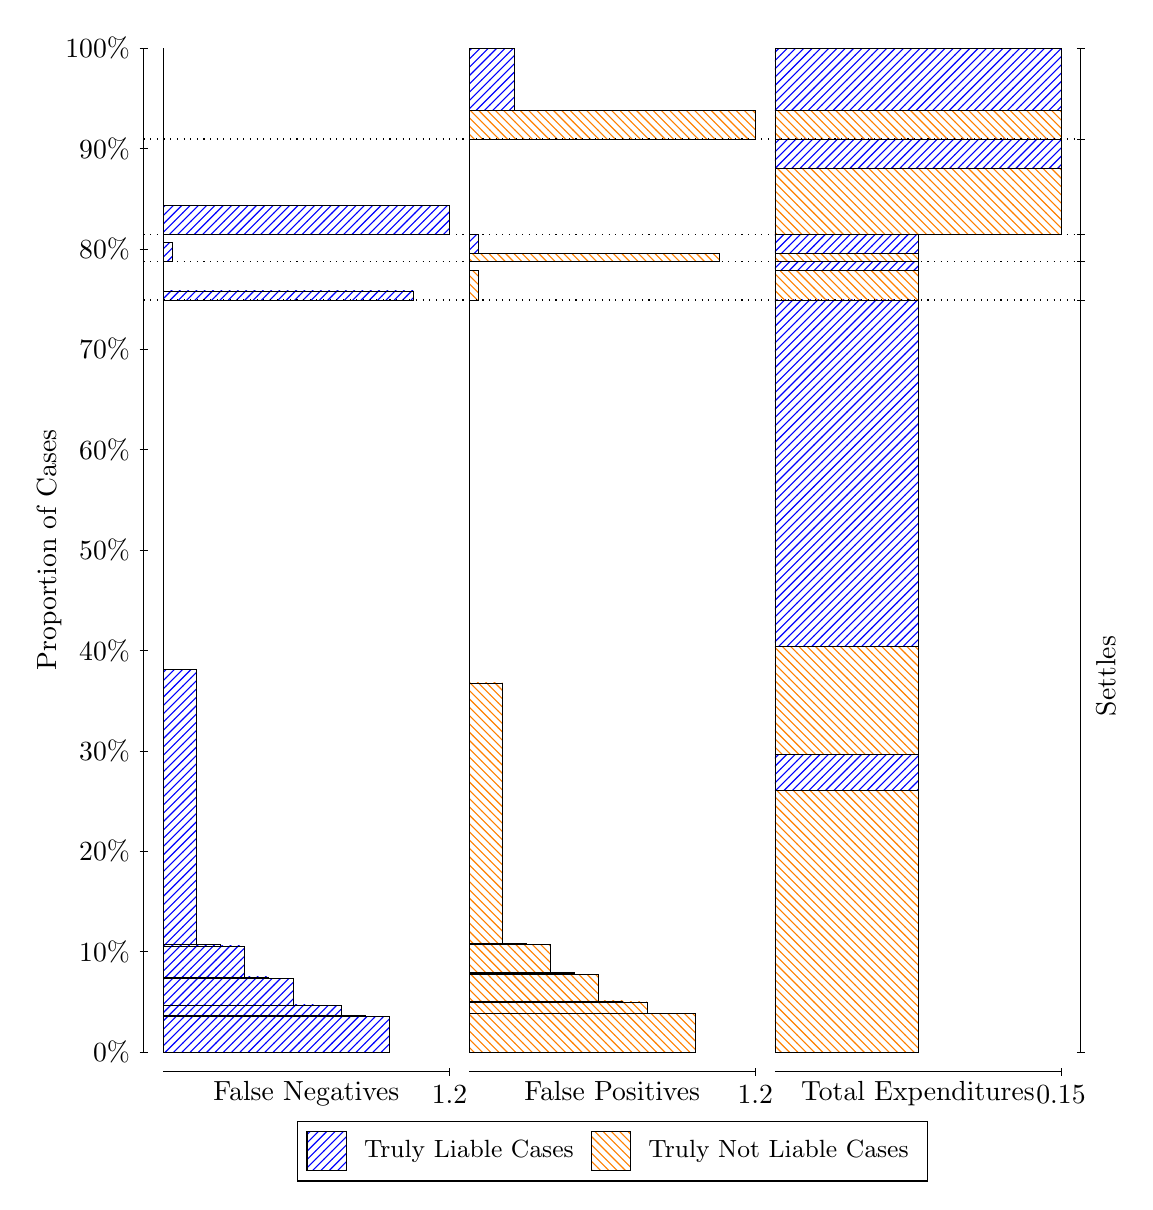
\begin{tikzpicture}
\draw[black, very thin] (1.5,1.75) -- (1.5,14.5);
\node[rotate=90, anchor=center] at (0.3, 8.125) {Proportion of Cases};
\draw[black, very thin] (1.45,1.75) -- (1.55,1.75);
\node[anchor=east] at (1.45, 1.75) {0\%};
\draw[black, very thin] (1.45,3.025) -- (1.55,3.025);
\node[anchor=east] at (1.45, 3.025) {10\%};
\draw[black, very thin] (1.45,4.3) -- (1.55,4.3);
\node[anchor=east] at (1.45, 4.3) {20\%};
\draw[black, very thin] (1.45,5.575) -- (1.55,5.575);
\node[anchor=east] at (1.45, 5.575) {30\%};
\draw[black, very thin] (1.45,6.85) -- (1.55,6.85);
\node[anchor=east] at (1.45, 6.85) {40\%};
\draw[black, very thin] (1.45,8.125) -- (1.55,8.125);
\node[anchor=east] at (1.45, 8.125) {50\%};
\draw[black, very thin] (1.45,9.4) -- (1.55,9.4);
\node[anchor=east] at (1.45, 9.4) {60\%};
\draw[black, very thin] (1.45,10.675) -- (1.55,10.675);
\node[anchor=east] at (1.45, 10.675) {70\%};
\draw[black, very thin] (1.45,11.95) -- (1.55,11.95);
\node[anchor=east] at (1.45, 11.95) {80\%};
\draw[black, very thin] (1.45,13.225) -- (1.55,13.225);
\node[anchor=east] at (1.45, 13.225) {90\%};
\draw[black, very thin] (1.45,14.5) -- (1.55,14.5);
\node[anchor=east] at (1.45, 14.5) {100\%};

\draw[black, very thin] (13.4,1.75) -- (13.4,14.5);
\draw[black, very thin] (13.35,1.75) -- (13.45,1.75);
\node[anchor=west] at (13.35, 1.75) {};
\draw[black, very thin] (13.35,11.3) -- (13.45,11.3);
\node[anchor=west] at (13.35, 11.3) {};
\draw[black, very thin] (13.35,11.794) -- (13.45,11.794);
\node[anchor=west] at (13.35, 11.794) {};
\draw[black, very thin] (13.35,12.135) -- (13.45,12.135);
\node[anchor=west] at (13.35, 12.135) {};
\draw[black, very thin] (13.35,13.345) -- (13.45,13.345);
\node[anchor=west] at (13.35, 13.345) {};
\draw[black, very thin] (13.35,14.5) -- (13.45,14.5);
\node[anchor=west] at (13.35, 14.5) {};

\draw[black, very thin, pattern color=blue, pattern=north east lines] (1.75,1.75) rectangle (4.6184,2.2056);
\draw[black, very thin, pattern color=blue, pattern=north east lines] (1.75,2.2056) rectangle (4.3125,2.2104);
\draw[black, very thin, pattern color=blue, pattern=north east lines] (1.75,2.2104) rectangle (4.0065,2.3376);
\draw[black, very thin, pattern color=blue, pattern=north east lines] (1.75,2.3376) rectangle (3.7005,2.3483);
\draw[black, very thin, pattern color=blue, pattern=north east lines] (1.75,2.3483) rectangle (3.3946,2.6832);
\draw[black, very thin, pattern color=blue, pattern=north east lines] (1.75,2.6832) rectangle (3.0886,2.7043);
\draw[black, very thin, pattern color=blue, pattern=north east lines] (1.75,2.7043) rectangle (2.7826,3.0971);
\draw[black, very thin, pattern color=blue, pattern=north east lines] (1.75,3.0971) rectangle (2.4767,3.1127);
\draw[black, very thin, pattern color=blue, pattern=north east lines] (1.75,3.1127) rectangle (2.1707,6.6118);
\draw[black, very thin, pattern color=orange, pattern=north west lines] (1.75,6.6118) rectangle (1.75,11.3);
\draw[black, very thin, pattern color=blue, pattern=north east lines] (1.75,11.3) rectangle (4.9244,11.416);
\draw[black, very thin, pattern color=orange, pattern=north west lines] (1.75,11.416) rectangle (1.75,11.794);
\draw[black, very thin, pattern color=blue, pattern=north east lines] (1.75,11.794) rectangle (1.8647,12.035);
\draw[black, very thin, pattern color=orange, pattern=north west lines] (1.75,12.035) rectangle (1.75,12.135);
\draw[black, very thin, pattern color=blue, pattern=north east lines] (1.75,12.135) rectangle (5.3833,12.501);
\draw[black, very thin, pattern color=orange, pattern=north west lines] (1.75,12.501) rectangle (1.75,13.345);
\draw[black, very thin, pattern color=orange, pattern=north west lines] (1.75,13.345) rectangle (1.75,13.711);
\draw[black, very thin, pattern color=blue, pattern=north east lines] (1.75,13.711) rectangle (1.75,14.5);
\draw[black, very thin, pattern color=orange, pattern=north west lines] (5.6333,1.75) rectangle (8.5018,2.236);
\draw[black, very thin, pattern color=orange, pattern=north west lines] (5.6333,2.236) rectangle (8.1958,2.2448);
\draw[black, very thin, pattern color=orange, pattern=north west lines] (5.6333,2.2448) rectangle (7.8898,2.3869);
\draw[black, very thin, pattern color=orange, pattern=north west lines] (5.6333,2.3869) rectangle (7.5839,2.3998);
\draw[black, very thin, pattern color=orange, pattern=north west lines] (5.6333,2.3998) rectangle (7.2779,2.7388);
\draw[black, very thin, pattern color=orange, pattern=north west lines] (5.6333,2.7388) rectangle (6.9719,2.7494);
\draw[black, very thin, pattern color=orange, pattern=north west lines] (5.6333,2.7494) rectangle (6.9719,2.7604);
\draw[black, very thin, pattern color=orange, pattern=north west lines] (5.6333,2.7604) rectangle (6.666,3.1196);
\draw[black, very thin, pattern color=orange, pattern=north west lines] (5.6333,3.1196) rectangle (6.36,3.131);
\draw[black, very thin, pattern color=orange, pattern=north west lines] (5.6333,3.131) rectangle (6.054,6.4385);
\draw[black, very thin, pattern color=blue, pattern=north east lines] (5.6333,6.4385) rectangle (5.6333,11.3);
\draw[black, very thin, pattern color=orange, pattern=north west lines] (5.6333,11.3) rectangle (5.7481,11.678);
\draw[black, very thin, pattern color=blue, pattern=north east lines] (5.6333,11.678) rectangle (5.6333,11.794);
\draw[black, very thin, pattern color=orange, pattern=north west lines] (5.6333,11.794) rectangle (8.8077,11.893);
\draw[black, very thin, pattern color=blue, pattern=north east lines] (5.6333,11.893) rectangle (5.7481,12.135);
\draw[black, very thin, pattern color=orange, pattern=north west lines] (5.6333,12.135) rectangle (5.6333,12.979);
\draw[black, very thin, pattern color=blue, pattern=north east lines] (5.6333,12.979) rectangle (5.6333,13.345);
\draw[black, very thin, pattern color=orange, pattern=north west lines] (5.6333,13.345) rectangle (9.2667,13.711);
\draw[black, very thin, pattern color=blue, pattern=north east lines] (5.6333,13.711) rectangle (6.207,14.5);
\draw[black, very thin, pattern color=orange, pattern=north west lines] (9.5167,1.75) rectangle (11.333,5.0689);
\draw[black, very thin, pattern color=blue, pattern=north east lines] (9.5167,5.0689) rectangle (11.333,5.5293);
\draw[black, very thin, pattern color=orange, pattern=north west lines] (9.5167,5.5293) rectangle (11.333,6.8989);
\draw[black, very thin, pattern color=blue, pattern=north east lines] (9.5167,6.8989) rectangle (11.333,11.3);
\draw[black, very thin, pattern color=orange, pattern=north west lines] (9.5167,11.3) rectangle (11.333,11.678);
\draw[black, very thin, pattern color=blue, pattern=north east lines] (9.5167,11.678) rectangle (11.333,11.794);
\draw[black, very thin, pattern color=orange, pattern=north west lines] (9.5167,11.794) rectangle (11.333,11.893);
\draw[black, very thin, pattern color=blue, pattern=north east lines] (9.5167,11.893) rectangle (11.333,12.135);
\draw[black, very thin, pattern color=orange, pattern=north west lines] (9.5167,12.135) rectangle (13.15,12.979);
\draw[black, very thin, pattern color=blue, pattern=north east lines] (9.5167,12.979) rectangle (13.15,13.345);
\draw[black, very thin, pattern color=orange, pattern=north west lines] (9.5167,13.345) rectangle (13.15,13.711);
\draw[black, very thin, pattern color=blue, pattern=north east lines] (9.5167,13.711) rectangle (13.15,14.5);
\draw[black, dotted] (1.5,11.3) -- (13.4,11.3);
\draw[black, dotted] (1.5,11.794) -- (13.4,11.794);
\draw[black, dotted] (1.5,12.135) -- (13.4,12.135);
\draw[black, dotted] (1.5,13.345) -- (13.4,13.345);
\draw[black, very thin] (1.75,1.5) -- (5.3833,1.5);
\node[anchor=north] at (3.5667, 1.5) {False Negatives};
\draw[black, very thin] (5.3833,1.45) -- (5.3833,1.55);
\node[anchor=north] at (5.3833, 1.45) {1.2};

\draw[black, very thin] (5.6333,1.5) -- (9.2667,1.5);
\node[anchor=north] at (7.45, 1.5) {False Positives};
\draw[black, very thin] (9.2667,1.45) -- (9.2667,1.55);
\node[anchor=north] at (9.2667, 1.45) {1.2};

\draw[black, very thin] (9.5167,1.5) -- (13.15,1.5);
\node[anchor=north] at (11.333, 1.5) {Total Expenditures};
\draw[black, very thin] (13.15,1.45) -- (13.15,1.55);
\node[anchor=north] at (13.15, 1.45) {0.15};

\node[black, centered, rotate=90] at (13.72, 6.5252) {Settles};





\draw (7.449999999999999,1.5) node[draw=none] (baseCoordinate) {};
\begin{scope}[align=center]
        \matrix[scale=0.5, draw=black, below=0.5cm of baseCoordinate, nodes={draw}, column sep=0.1cm]{
            \node[rectangle, draw, minimum width=0.5cm, minimum height=0.5cm, pattern=north east lines, pattern color=blue] {}; &
            \node[draw=none, font=\small] (B) {Truly Liable Cases}; &
            \node[rectangle, draw, minimum width=0.5cm, minimum height=0.5cm, pattern=north west lines, pattern color=orange] {}; &
            \node[draw=none, font=\small] (B) {Truly Not Liable Cases}; \\
            };
\end{scope}

\end{tikzpicture}
\end{document}